\subsection{adjustbox: adjust boxed content}
\begin{verbatim}
\usepackage{adjustbox}
...
\begin{adjustbox}{
  max totalsize={\textwidth}{\textheight},center}
\end{adjustbox}
\end{verbatim}

\subsection{minipage}
\begin{minipage}[c]{3cm}
  \lipsum[][1-3]
\end{minipage}
\begin{minipage}[c]{3cm}
  \begin{verbatim}
\begin{minipage}[c]{3cm}
  \lipsum[][1-3]
\end{minipage}
  \end{verbatim}
\end{minipage}

\subsection{Beamer class}
\subsubsection{Accessing section names}
\verb |\secname|\\
\verb |\subsecname|\\
\subsubsection{Animations}
Use \verb|%| at the end of the line to avoid interpeting new line causing x-shift in the animation:
\begin{verbatim}
\includegraphics<1>[height=0.5\textheight]{figures/1.pdf}%
\includegraphics<2>[height=0.5\textheight]{figures/2.pdf}
\end{verbatim}
\verb|\visible<3>{...}| Put a set of command visible only on slide 3
\subsubsection{Custom footer}
\begin{verbatim}
\newcommand{\secfoot}{
\begin{tikzpicture}[remember picture, overlay]
  \node [anchor=south,node font=\tiny,text=blue!50] (node1) at (current page.south) [] {\secname/\subsecname};
\end{tikzpicture}
}
\end{verbatim}

\subsection{LaTeX default colors -- xcolor package --}
\begin{center}
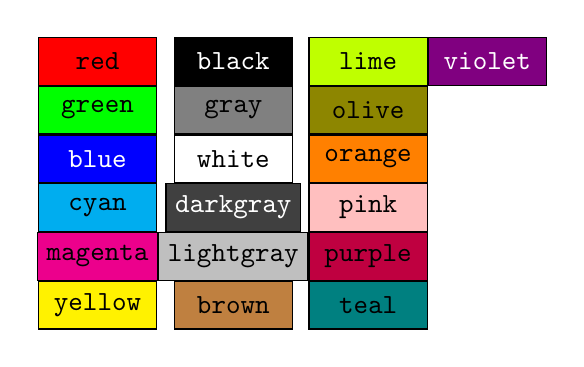
\begin{tikzpicture}[c/.style={minimum width=1.5cm,minimum height=4ex,rectangle,draw}]
  \matrix{
    \node[c,fill=red]{\verb|red|}; &&
    \node[c,fill=black,text=white]{\verb|black|}; &&
    \node[c,fill=lime]{\verb|lime|}; &&
    \node[c,fill=violet,text=white]{\verb|violet|}; \\
    \node[c,fill=green]{\verb|green|}; &&
    \node[c,fill=gray]{\verb|gray|}; &&
    \node[c,fill=olive]{\verb|olive|}; \\
    \node[c,fill=blue,text=white]{\verb|blue|}; &&
    \node[c,fill=white]{\verb|white|}; &&
    \node[c,fill=orange]{\verb|orange|}; \\
    \node[c,fill=cyan]{\verb|cyan|}; &&
    \node[c,fill=darkgray,text=white]{\verb|darkgray|}; &&
    \node[c,fill=pink]{\verb|pink|}; \\
    \node[c,fill=magenta]{\verb|magenta|}; &&
    \node[c,fill=lightgray]{\verb|lightgray|}; &&
    \node[c,fill=purple]{\verb|purple|}; \\
    \node[c,fill=yellow]{\verb|yellow|}; &&
    \node[c,fill=brown]{\verb|brown|}; &&
    \node[c,fill=teal]{\verb|teal|}; \\
  };
\end{tikzpicture}
\end{center}
